\chapter{Data Engineering Pipeline and Knowledge Graph Construction}
\label{ch:pipeline}
\minitoc

\section*{Introduction}
\addcontentsline{toc}{section}{Introduction}

This chapter details the transformation of the source document into queryable data. It discusses the selected processing environment, outlines the design of the extraction pipeline, and explicates the transformations implemented at each stage. Additionally, it presents the validated node set generated and the knowledge graph constructed from it, concluding with an evaluation of the pipeline's performance and its remaining limitations.

\section{Processing Environment}

Before describing the pipeline itself, it is worth justifying the kind of pipeline it is.
Three choices were made before any extraction rule was written: a deterministic, rule-based
approach over a learned one, a single-process program over a distributed framework, and a
specific set of libraries chosen against the constraints of Table~\ref{tab:constraints}.

\subsection{Motivation for a Deterministic, Rule-Based Pipeline}

An alternative strategy for addressing this extraction challenge involves training a model by annotating a selection of pages to classify text regions and subsequently generalizing from this information. However, this approach was ultimately dismissed for practical reasons prior to any principled considerations. Specifically, the absence of annotated data posed significant hurdles, as the effort required to produce sufficient annotations for a single seventy-nine-page document would have outweighed the efforts involved in crafting a set of rules, all while complicating verifiability.

Verifiability serves as the foundational rationale for adopting a rule-based approach. Rules derived from measured character geometry can be readily verified against the originating page. In instances of failure, such discrepancies can be inspected closely, and the necessary corrections are localized. Conversely, a learned region classifier that misinterprets a single table offers no comparable insight into its decision-making process. In documents where errors are subtle and plausible, the ability to elucidate the reasoning behind a character's interpretation holds greater value than the enhanced flexibility that a learned approach might provide.

\subsection{Why Not a Distributed Processing Framework}

Distributed frameworks, such as Apache Spark, are typically employed when data processing demands exceed the capabilities of a single machine. However, this particular scenario is not one of those cases. The complete document is only a few megabytes, and the subset processed yields 327 records, with a full reconstruction of the knowledge base requiring approximately fifteen to twenty seconds on an average laptop.

Implementing a distributed framework would introduce unnecessary complexities, such as an execution model, cluster configuration, and serialization boundaries, which are irrelevant to this problem. The primary challenge lies in the interpretative aspect, specifically in discerning the meanings of characters rather than in the rapid processing of numerous characters. Consequently, the pipeline is structured as a single-pass, single-process program, which is best suited for this task and facilitates inspection of intermediate outputs during development.

\subsection{Libraries Selected for Extraction, Validation and Modelling}

Extraction is facilitated by pdfplumber\citep{pdfplumber}, which provides detailed information about characters and words, including their coordinates, font names, and sizes. This character-level access is essential, as the superscript rule discussed in Chapter 2 relies on the vertical offset and size of individual characters, making ware-level output insufficient.

The node model is established using Pydantic\citep{pydantic_docs}, ensuring that structural expectations are strictly enforced during construction. Consequently, any record that omits a required field or contains an authority code outside the recognized set will fail promptly, preventing issues from arising later in the graph.

\section{Pipeline Design}

With the environment settled, the pipeline itself has a shape worth laying out: how many
stages it has, what each one hands to the next, and how the code implementing it is
organised into modules.

\subsection{Global Architecture}

The process pipeline is made up of eight consecutive processes, where each process takes input from its previous process, and each process can be inspected independently. The raw characters get converted to physical rows, the physical rows are grouped into task blocks, the task blocks are cleaned and enriched with geometric and role-based data, and finally, they are arranged into validated records.
Figure~\ref{fig:pipeline} shows the pipeline end to end, and it is worth reading it as a
progressive narrowing of interpretation rather than as a sequence of transformations. At
the left-hand edge the input is a stream of glyphs with coordinates, carrying no notion of
a row, a cell, an activity or a role: the PDF format records where ink was placed, not what
the ink means. At the right-hand edge the output is a set of validated records in which
every responsibility is an explicit assertion that a named role holds a named obligation
over a named activity. Every stage in between recovers exactly one layer of structure that
the printed page expresses visually and the file itself does not encode.

The ordering is not arbitrary, and the stages are not independent. Each one consumes an
abstraction the previous stage established and would be meaningless without it: codes
cannot be separated from footnote markers before there are cells to inspect, cells cannot
be attributed to roles before the rotated column headers have been clustered into columns,
and no activity can be assembled before its block boundaries are known. This dependency is
the reason the pipeline is deterministic and staged rather than a single extraction pass.
A failure at any stage is therefore localised to that stage and inspectable in isolation,
which is what made the defects catalogued in Chapter~\ref{ch:datasource} diagnosable at
all.

\begin{figure}[htbp]
\centering
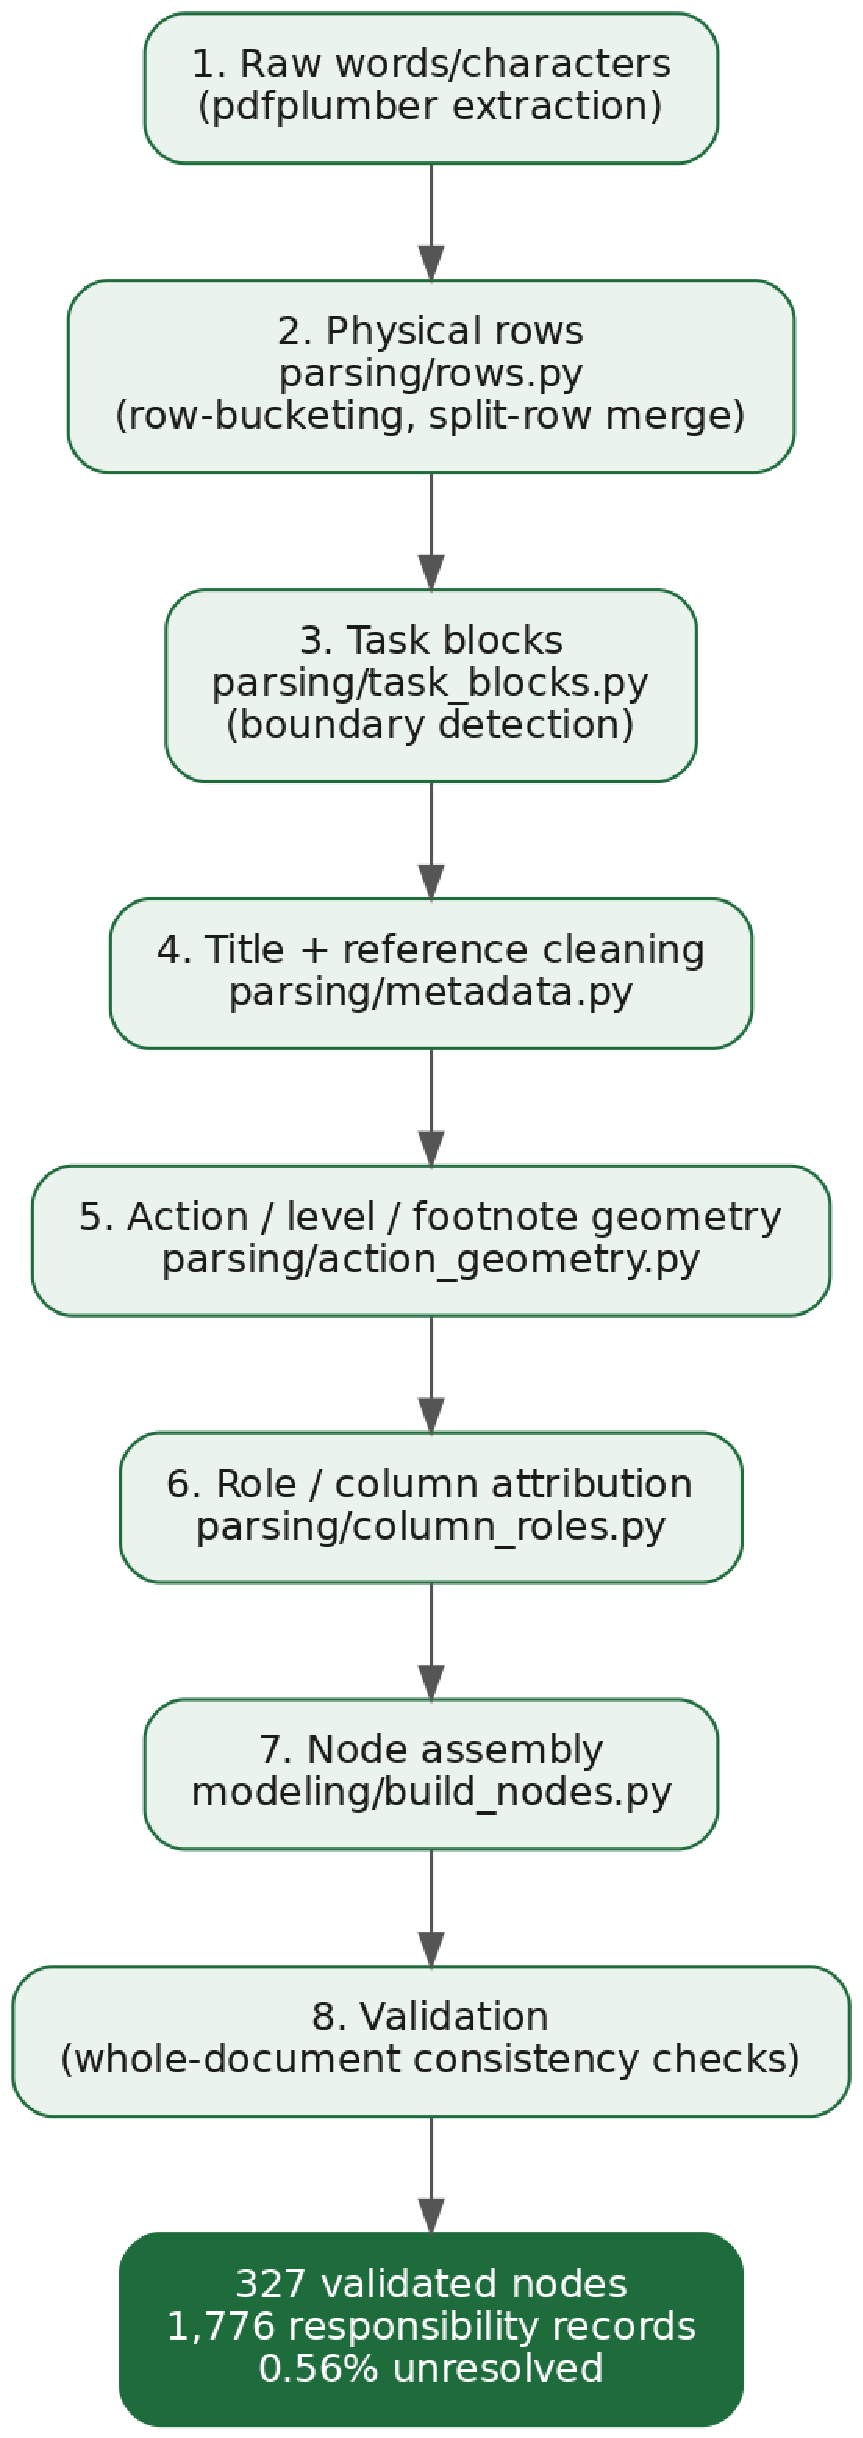
\includegraphics[width=0.94\textwidth,height=0.88\textheight,keepaspectratio]{figures/fig2_pipeline.pdf}
\caption{Eight-stage data engineering pipeline, from raw PDF extraction to a validated node set.}
\label{fig:pipeline}
\end{figure}

Table~\ref{tab:stages} names each stage, states what it does, and records why it exists at all, since several of them were added only after a specific defect made their absence visible.

\begin{longtable}{|p{0.045\textwidth}|p{0.19\textwidth}|p{0.32\textwidth}|p{0.30\textwidth}|}
\caption{Stages of the data engineering pipeline, with the motivation for each.}\label{tab:stages}\\
\hline
\rowcolor{myblue}\textcolor{white}{\textbf{\#}} & \textcolor{white}{\textbf{Name}} & \textcolor{white}{\textbf{Function}} & \textcolor{white}{\textbf{Why it exists}} \\
\hline
\endfirsthead
\hline
\rowcolor{myblue}\textcolor{white}{\textbf{\#}} & \textcolor{white}{\textbf{Name}} & \textcolor{white}{\textbf{Function}} & \textcolor{white}{\textbf{Why it exists}} \\
\hline
\endhead
1 & Raw extraction & Characters and words with coordinates, fonts, and sizes are read from the PDF. & Page-level text extraction discards the geometry on which every later stage depends, so extraction had to be character-level from the outset. \\ \hline
2 & Row reconstruction & Words are grouped into physical rows by vertical alignment, with split rows merged where the merge is provably safe. & Activities in the Non-Sovereign Operations chapter are printed across two physical rows, and without merging they were parsed as two unrelated fragments. \\ \hline
3 & Task block detection & Rows are grouped into task blocks, and boundaries between consecutive activities are determined. & A title wrapping past its own identifier row was being claimed by the following activity, which silently attached responsibilities to the wrong task. \\ \hline
4 & Title and reference cleaning & Titles are normalised, cross-references are extracted and expanded, footnote digits are stripped from title text. & Roughly a quarter of titles carried embedded reference phrases or stray digits, which corrupted the search index and made free-text resolution unreliable. \\ \hline
5 & Geometric attribution & Authority codes are separated from footnote markers by character geometry, and levels are attached. & A code and a footnote marker are both a letter beside a digit; only font size and vertical offset distinguish them, so fusing the two inverted the meaning of the cell. \\ \hline
6 & Role attribution & Codes are matched to roles by horizontal alignment with clustered, rotated column headers. & Column headers are printed rotated through ninety degrees and are not recoverable as table headers, so columns had to be reconstructed from header coordinates. \\ \hline
7 & Node assembly & Enriched blocks are validated against the schema and merged with the chapter and process skeleton. & Enforcing the schema at construction makes a malformed record fail immediately, rather than surfacing later as a wrong answer to a user. \\ \hline
8 & Validation & Whole-document consistency checks are run across the assembled node set. & Per-record validity does not imply document-level coherence: orphaned identifiers and unresolved references are only visible once the full set exists. \\ \hline
\end{longtable}

\subsection{Data Flow and Modular Organisation}

The process is performed in each individual module with well-defined boundaries such that if an error occurs, it will be easier to pinpoint exactly where it occurred based on the output of one particular stage as opposed to following the execution throughout the whole program. This factor had great significance throughout the development process because whenever an incorrect output came out, the first thing to consider was which stage produced it.

Modules for parsing take care of rows, action blocks, metadata, geometry of action, column definitions, and text cleaning. Modules for modelling handle nodes, structural backbone, graph, and caching. The schema lives in a separate module, which is dependent on both but depends on none of the two.

\section{Data Ingestion}

The ingestion process deals with each page of the document individually. Characters and their locations and font metrics, as well as words with their bounding boxes are extracted from every single page. These two granularities are saved because the row construction needs word granularity, and the superscript rule is based on the character granularity.

References are extracted independently from other pages of the same document. The legend of authority codes is converted into a structured file that describes the full code, its hierarchy level and the meaning. This reference is checked against the schema and seventeen entries are loaded successfully. Abbreviations are extracted as a glossary. The glossary needed a special approach due to the facts that some entries break a line, some rows are section headings but not the definitions and the term and its definition are sometimes placed with a fractional difference in point. Therefore, row grouping is done with the same tolerance as elsewhere in the processing.

\section{Document Processing and Normalisation}

Stages two through six of Table~\ref{tab:stages} are covered here: the point where raw
characters become rows, rows become task blocks, and blocks are cleaned and enriched enough
for a schema to accept them. This is also where most of the defects catalogued in
Chapter~\ref{ch:datasource} are addressed directly, one subsection per family of defect.

\subsection{Row Reconstruction}

Words are arranged into lines through grouping of their vertical coordinates. The reason for tolerance is that text that may appear on the same visual line is normally not placed on identical coordinates. Where the chapter Non-sovereign operations splits a logical line into two lines, these lines are combined into one only when the specific condition described in Chapter 2 applies. That is, the lower line consists of authority codes alone.

\subsection{Task Block Detection}

Blocks then come out of rows in such a way that each block represents an activity. The boundary detection turned out to be the most iterative part of the process as the visual cue that denotes a boundary was unreliable. There were three different cues considered: (1) whether there is an open task, (2) whether the open task ends on a full stop, and (3) whether there is any new row with authority codes while there are codes for the current open task. Of these three cues, the third one appears to be the most reliable one.

\subsection{Title and Reference Cleaning}

Normalization of titles is achieved by stripping footnote digits, compressing whitespace, and stripping references that would have been incorporated as noise in the title. Extraction of references is concentrated in one function used by all pathways that deal with titles or notes. The current scheme contrasts with the original design that had two different but conflicting implementations, one of which could handle the reference pattern while the other could not.

\subsection{Geometric Attribution of Authority Codes}

Codes of authority are found in each row and are distinguished from footnote indicators according to the character-level rule stated in Chapter 2. Level digits belonging to the codes remain intact as part of the code, but superscripted digits are entered independently as footnote numbers for that responsibility.

\subsection{Role Attribution}

The enriched blocks are put together in such a way that the records follow the required schema and they get coupled with a structural skeleton that contains the chapter nodes and process nodes, since these nodes are containers for the records and not emitted as activities by the table parser.

The parentage is defined explicitly and not by the structure of the identifiers. There is a pointer to the parent node inside each record and the hierarchy is built using these pointers. In an older version of the system, the children of a node were defined based on the structure of the identifier and it worked well only for two of the four levels but not for the other two levels. This problem was detected only when the threshold variants started appearing in the identifier space and the grandchildren were clashing with the children under the same prefix.

The indicators in Table~\ref{tab:quality} are the measured state of the node set after construction, and they are the figures against which the pipeline's adequacy is judged.

\begin{longtable}{|p{0.52\textwidth}|p{0.34\textwidth}|}
\caption{Data quality indicators after node construction.}\label{tab:quality}\\
\hline
\rowcolor{myblue}\textcolor{white}{\textbf{Indicator}} & \textcolor{white}{\textbf{Value}} \\
\hline
\endfirsthead
\hline
\rowcolor{myblue}\textcolor{white}{\textbf{Indicator}} & \textcolor{white}{\textbf{Value}} \\
\hline
\endhead
Structured records produced & 327 \\ \hline
Responsibility entries extracted & 1,776 \\ \hline
Distinct roles identified & 131 \\ \hline
Unresolved role entries & 10 (0.56\%) \\ \hline
Average responsibilities per record & 5.48 \\ \hline
Records with no direct responsibilities & 29.63\% \\ \hline
Cross-references captured & 14 \\ \hline
Responsibility entries carrying footnote references & 113 (6.36\%), across 44 records \\ \hline
Residual title corruption & 1 record (2.222.1) \\ \hline
\end{longtable}

\subsection{Geometric Tolerances}
\label{sec:geotolerances}

Several pipeline stages reason about position and size rather than about text, because the
distinctions they draw are not present in the character stream at all. Those stages are
governed by the tolerances in Table~\ref{tab:geoparams}, stated in PDF user-space units,
where one unit is $1/72$ of an inch. The values are recorded here because without them the
extraction is not reproducible: the same source document processed with different tolerances
yields a different node set.

\begin{longtable}{|p{0.26\textwidth}|p{0.09\textwidth}|p{0.51\textwidth}|}
\caption{Geometric tolerances governing extraction, in PDF user-space units.}\label{tab:geoparams}\\
\hline
\rowcolor{myblue}\textcolor{white}{\textbf{Tolerance}} & \textcolor{white}{\textbf{Value}} & \textcolor{white}{\textbf{What it separates}} \\
\hline
\endfirsthead
\hline
\rowcolor{myblue}\textcolor{white}{\textbf{Tolerance}} & \textcolor{white}{\textbf{Value}} & \textcolor{white}{\textbf{What it separates}} \\
\hline
\endhead
Body text minimum size & $8.0$ & Characters at or above this size are body text. Below it, a character is a candidate footnote marker rather than content. \\ \hline
Footnote digit maximum size & $4.0$ & A trailing digit at or below this size is treated as a footnote reference and stripped from the cell. \\ \hline
Row band padding & $1.0$ & Vertical tolerance when collecting the characters and words belonging to one printed row. \\ \hline
Row merge maximum gap & $5.0$ & Two vertically adjacent row bands closer than this may be merged into a single logical row. \\ \hline
Column alignment tolerance & $2.0$ & Horizontal distance within which a cell is considered aligned to a column centre. \\ \hline
Tight cluster gap & $3.0$ & Characters separated by less than this belong to the same header cluster. \\ \hline
Column merge gap & $14.0$ & Two header clusters closer than this are treated as one column rather than two. \\ \hline
Subgroup tolerance & $0.6$ & Vertical agreement required for header fragments to form one subgroup. \\ \hline
Subgroup minimum gap & $1.5$ & Separation below which two candidate subgroups are not distinguished. \\ \hline
Decoration gap maximum & $8.0$ & Distance beyond which an adjacent glyph is ruled out as decoration attached to a code. \\ \hline
Spaced-word gap maximum & $6.0$ & Gap below which adjacent single letters are read as letter-spaced prose rather than as standalone codes. \\ \hline
Glossary title minimum size & $20$ & Font size at or above which a glossary line is a heading rather than an entry. \\ \hline
Glossary top merge tolerance & $3.0$ & Vertical tolerance when joining a wrapped glossary definition to its term. \\ \hline
\end{longtable}

Two of these tolerances resolve ambiguities that no single test settles on its own.

The footnote-digit rule is size-based, and size alone produces false positives. Department
codes such as \texttt{PGCL.1}, \texttt{FIFC.4} and \texttt{FITR.2} also end in a digit, and
that digit belongs to the code. The rule therefore carries a second, independent condition:
the character preceding the digit must not be a period. The two tests are needed together
because the same code was observed rendering its digit at normal size on some pages and at
the reduced footnote size on others, so size is not a reliable discriminator by itself.

The spaced-word tolerance separates a genuine authority code from letter-spaced prose. A
single capital letter standing alone in a row may be an authority code, or it may be one
glyph of a title that the renderer has spaced out character by character, as in
\texttt{A p p r a i s a l}. A real code is followed either by the gap to the next table
column or by nothing at all, so adjacency below $6.0$ units to another single-letter word
identifies the second case. Authority codes themselves are recognised by the pattern
\texttt{\^{}[ICRA]\textbackslash d*\$}, one of the four letters with an optional level digit.

\begin{figure}[htbp]
\centering
% ---------------------------------------------------------------
% PLACEHOLDER — replace with an annotated page crop showing the
% geometry: column header clusters, the alignment band for one
% column, a normal-size code beside a reduced-size footnote digit.
% Suggested filename: figures/fig3_geometry_annotated.png
% ---------------------------------------------------------------
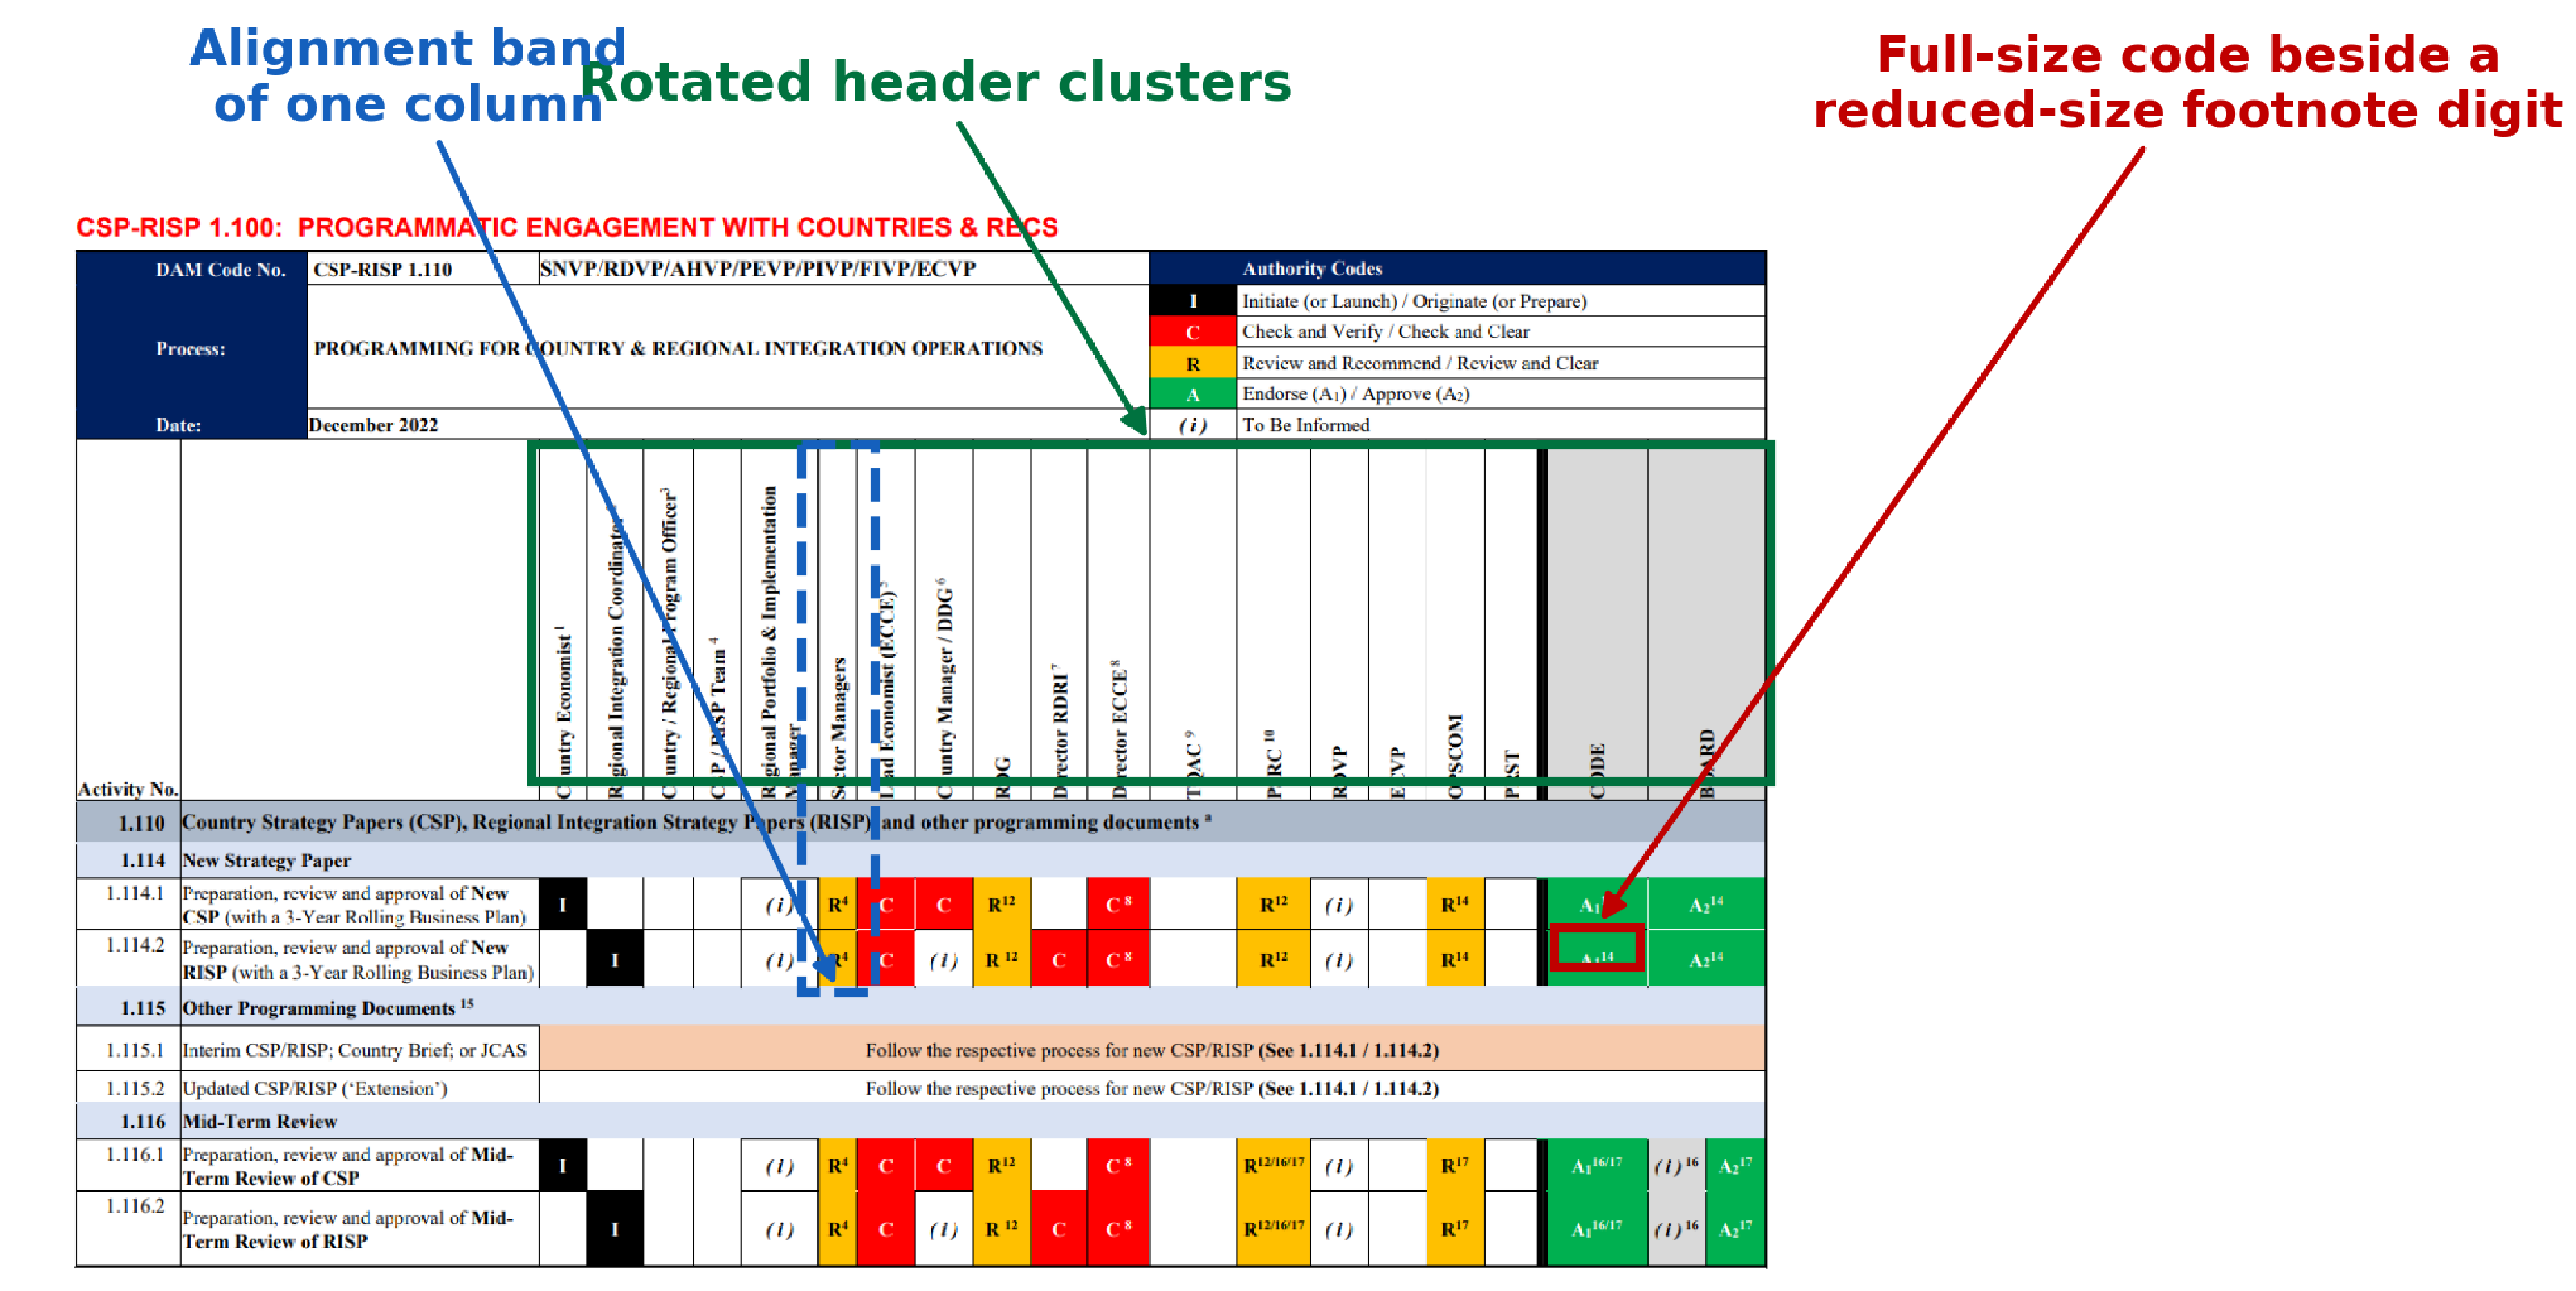
\includegraphics[width=0.95\textwidth]{figures/fig3_geometry_annotated.pdf}
\caption{A DAM table region annotated with the geometric quantities used during extraction:
rotated header clusters, the horizontal alignment band of one column, and a full-size
authority code beside a reduced-size footnote digit.}
\label{fig:geoannotated}
\end{figure}

Figure~\ref{fig:geoannotated} shows these quantities on a real page region.

\section{Knowledge Graph Modelling}

The pipeline's final output is a validated set of nodes, but a set on its own cannot answer
a relational question such as who approves an activity. That is why the nodes are loaded
into a graph rather than kept flat, with the graph's nodes and edges defined next, along
with what the assembled structure looks like in aggregate.

\subsection{Why a Graph}

The valid set of nodes could have been modeled as either relational tables or as a flat set of documents\citep{hogan2021kg}. The graph was chosen since the queries posed to the system are relational in nature. For instance, the query "Who approves this activity" translates into traveling in the graph from the activity node via edges of a certain kind, while "which activities does this role approve" amounts to traveling the opposite way in the graph. In both instances, the operation performed is a single one on a graph, unlike join or scan on a flat structure.

A directed multigraph is used instead of a simple graph since one role can hold multiple responsibilities for the same activity. That is why two nodes will be linked with multiple edges, each carrying its unique authorization code and references to the footnote.

\subsection{Node and Edge Schema}

The graph contains two kinds of node. Activity nodes correspond one-to-one with the 327 structured records. Role nodes correspond to the 131 distinct roles. Edges carry the relationships between them.

Table~\ref{tab:edges} sets out the edge types the graph carries and what each one asserts.

\begin{longtable}{|p{0.24\textwidth}|p{0.24\textwidth}|p{0.42\textwidth}|}
\caption{Edge types in the knowledge graph.}\label{tab:edges}\\
\hline
\rowcolor{myblue}\textcolor{white}{\textbf{Edge type}} & \textcolor{white}{\textbf{From $\rightarrow$ To}} & \textcolor{white}{\textbf{Meaning}} \\
\hline
\endfirsthead
\hline
\rowcolor{myblue}\textcolor{white}{\textbf{Edge type}} & \textcolor{white}{\textbf{From $\rightarrow$ To}} & \textcolor{white}{\textbf{Meaning}} \\
\hline
\endhead
\texttt{contains} & Activity $\rightarrow$ Activity & Hierarchical containment: chapter to process, process to task, task to child task or threshold variant. \\ \hline
\texttt{responsible\_for} & Role $\rightarrow$ Activity & A recorded responsibility, carrying the authority code, its level, and any footnote references. \\ \hline
\texttt{references} & Activity $\rightarrow$ Activity & A cross-reference extracted from the activity's own text, including ranges expanded to their members. \\ \hline
\end{longtable}

Figure~\ref{fig:graph} shows a representative excerpt, centred on activity 3.111, in which the containment edge from the parent process and the individual responsibility edges to each role are both visible.

\begin{figure}[htbp]
\centering
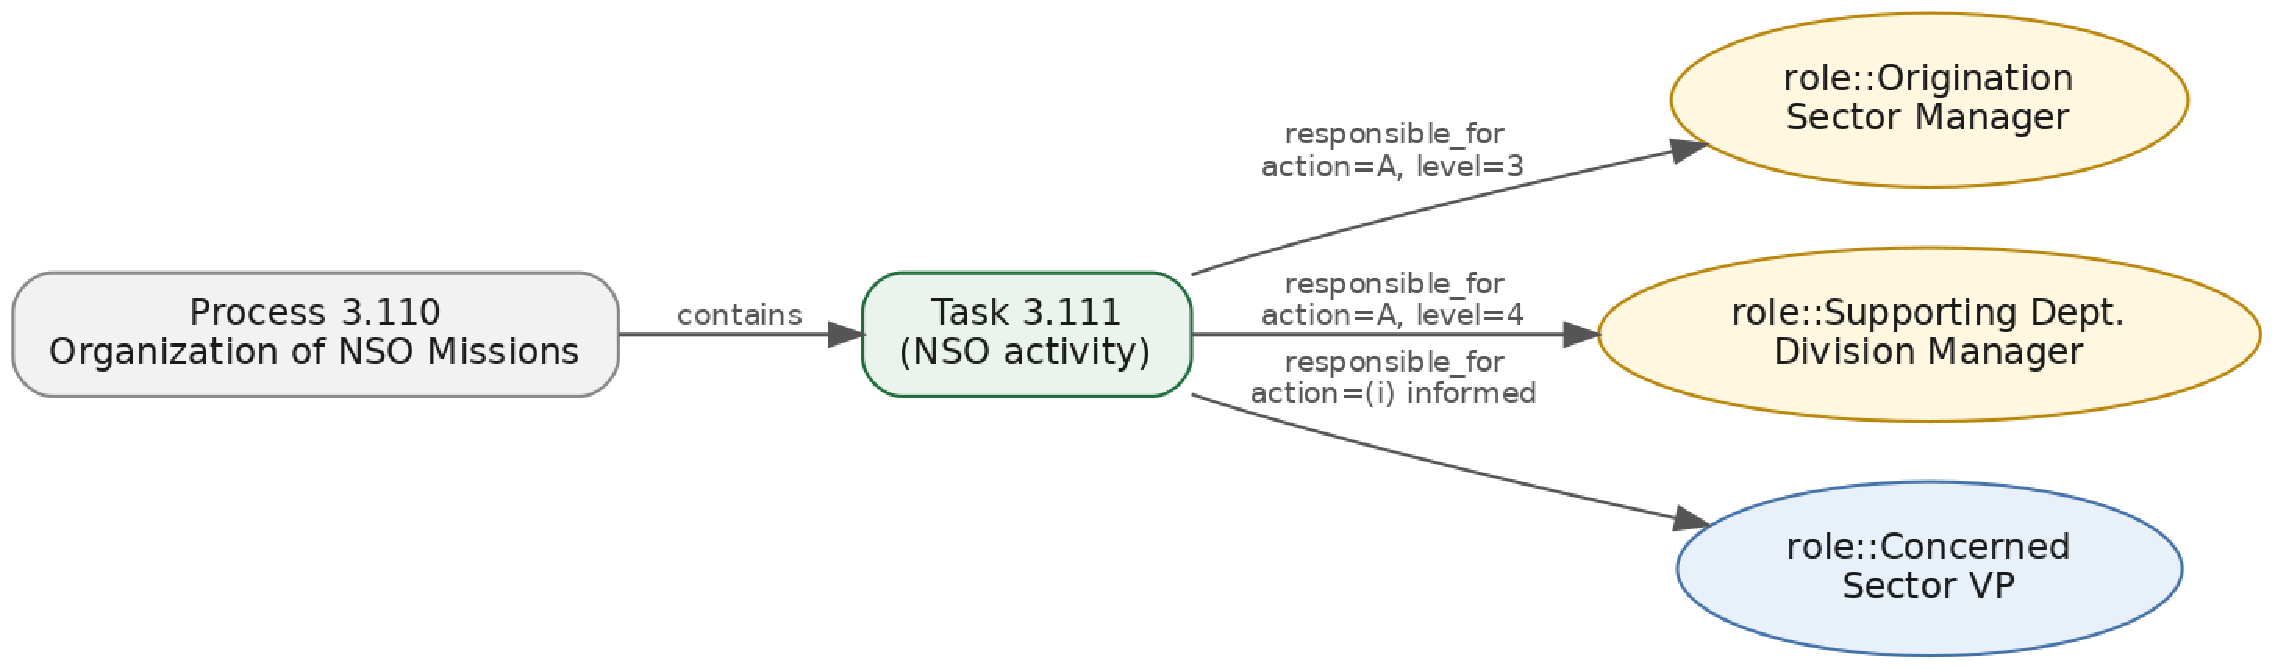
\includegraphics[width=0.94\textwidth,height=0.88\textheight,keepaspectratio]{figures/fig3_graph.pdf}
\caption{Excerpt of the knowledge graph around activity 3.111, showing the containment edge from its parent process and the responsibility edges connecting it to its approving and informed roles.}
\label{fig:graph}
\end{figure}

\subsection{Graph Statistics}

The assembled graph holds 459 nodes and 2,108 edges. The node count is the sum of the 327 activities and the 131 roles, plus one aggregate node. The edge count is dominated by responsibility edges, with containment edges accounting for the hierarchy and a small number of reference edges added from cross-references.

\section{Pipeline Evaluation}

A pipeline that runs is not the same as one that can be trusted. Both the extraction step's
runtime behaviour and the data-quality checks applied to its output are covered below, since
output is not allowed anywhere near a user's question until it passes them.

\subsection{Execution and Caching}

It takes around fifteen to twenty seconds to reconstruct the document from the PDF. This time frame is fine in an offline scenario but unacceptable when requested; hence, the node set that is being built is written into a cache file and later read during application initialization. The service running will never access the PDF while working.

The above arrangement deviates from the original one; the explanation for this change is provided in Chapter 5. The original implementation started by parsing the document when the application was initialized and was halted by the hosting system because of memory limit issues. Caching solved this problem, and in addition, this change prevented a more hidden problem, which is relying on the runtime environment to parse the document.

\subsection{Data Quality Outcomes}

The role that is unresolved For the subset that was processed, there are missing titles in record 2.516 and record 2.522, and one record (2.222.1) remains partially corrupted. Rather than being accepted and unstated, all three are known and documented. There was a candidate fix for the last case that was applied and tested but found to be not a fix for the target case but a regression in another case, so it was reverted. This was thought to be a better result than to leave a documented defect where a change could be made to make the overall extraction more desirable.

The second restriction is further discussed in the general conclusion and is due to the footnotes. Footnote reference numbers are captured and remain unchanged in respect of responsibilities and the bottom of the page text will not yet be parsed so that the system can say that a qualification is applicable if the text says so. During testing two similar extraction defects were found: a column header was confused as a role name, while two adjacent footnote digits were joined into one number in the same records. The planned remediation is also documented along with these two in Chapter~5.

But only three chapters have been exercised against the pipeline. The remainder of the entire document has the same table conventions as far as the present document is concerned, but for purposes of this document, at least, and certainly as part of a continuation of the work, such tables would be the first step in processing them.ved at a rate of 0.56 percent is the key quality measure of the pipeline and deserves careful consideration. This rate is the ratio of the number of responsibility items extracted, for which there was no matching column header. This is not related to checking whether the right code has been extracted for each cell, and this is an assessment that can only be done manually because of the lack of a ground truth dataset. This issue was examined by sampling and comparing particular activities against the printed page.

\subsection{Observed Limitations}

For the subset that was processed, there are missing titles in record 2.516 and record 2.522, and one record (2.222.1) remains partially corrupted. Rather than being accepted and unstated, all three are known and documented. There was a candidate fix for the last case, that was applied, tested, but found to be not a fix for the target case but a regression in another case so it was reverted. This was thought to be a better result than to leave a documented defect where a change could be made to make the overall extraction more desirable.

The second restriction is further discussed in the general conclusion and is due to the footnotes. Footnote reference numbers are captured, and remain unchanged in respect of responsibilities and the bottom of the page text will not yet be parsed so that the system can say that a qualification is applicable if the text says so. During testing two similar extraction defects were found: a column header was confused as a role name while two adjacent footnote digits were joined into one number in the same records. The planned remediation is also documented along with these two in Chapter~5.

But only three chapters have been exercised against the pipeline. The remainder of the entire document has the same table conventions as far as the present document is concerned but for purposes of this document, at least, and certainly as part of a continuation of the work, such tables would be the first step in processing them.

\section*{Conclusion}
\addcontentsline{toc}{section}{Conclusion}
The pipeline transforms a low-level document that is only graphically organized into 327 records that are validated and have 1776 responsibility entries, with less than 1 percent of those entries unassigned, and it converts the output into a graph of 459 nodes and 2108 edges that can answer questions about relations by traversal. Each stage is deterministic and inspectable, which enabled the defects as described in Chapter~2 to be detected, corrected, and staved off. The next chapter adds the agent that queries this graph.